\chapter{Collaboration}

In this chapter, we will introduce different types of collaborative methods. People will continue to interact in new and different ways. One outcome of the marriage between technology and communication is a technical workplace. The study of such workplaces gives rise to a new field: \textit{Computer-Supported Cooperative Work} (CSCW). CSCW analyzes the way groups work and seeks to discover how technology can help them work. Sometimes we refer to CSCW as \textit{groupware}. Often this term is used synonymously with CSCW technology. However, this is not completely true. In the following sections, we will define the exact definition of groupware and CSCW applications. We will also create a taxonomy of groupware and compare this taxonomy to CSCW applications. There exists another collaborative method, especially targeted at collaborative learning, \textit{Computer-Supported Collaborative Learning} (CSCL). This collaborative method is a refinement of CSCW. 
\\ \\
The second part of this chapter defines the collaborative patterns typically used in a collaborative application (whether it is defined as groupware, CSCW or CSCL). We finish this chapter with a collaboration stack that defines the different levels in collaborative application.

\section{Groupware}

\subsection{Definition}

There exist several definitions for groupware. Some define groupware as collaborative software for small focused groups, that do not give organization-wide support. Another definitions says that groupware can be viewed as the class of applications arising from the merging of computers and large information bases and communications technology. These applications may or may not specifically support cooperation. Ellis et al define groupware as follows:
\begin{mydef}
\textbf{Groupware}. computer-based systems that support groups of people engaged in a common task (or goal) and that provide an interface to a shared environment. \cite{groupware}
\end{mydef}
In this definition, the writer uses the notions of \textit{common task} and \textit{shared environment}. This definition excludes multi-user environments where people do not share a common task. Moreover, the definition does not require users to be active at the same time. We can make a distinction between \textit{real-time groupware} and \textit{non-real-time groupware}. Our modeling framework tries to support both real-time as well as non-real-time groupware.
\\ \\
Furthermore, we can argue what distinguishes groupware from non-groupware. According to Koch, '\textit{the core characteristic of groupware is the non-separation or non-isolation of users from each other. Groupware explicitly provides awareness of the co-workers and their activities and does not separate the users from each other as it is common in distributed systems in general.}' \cite{CSCWConcepts}.

\subsection{Communication, Collaboration and Coordination}

A groupware application does not only support interactions between a user and the system. Its main strength is the interaction among users, moreover group interactions. As we focus on how to support this group interaction, we must address issues in three areas: communication, collaboration and coordination.
\\ \\
The main problem we currently stumble upon in collaborative applications is the separation of synchronous and asynchronous communication. For instance, asynchronous communication such as electronic mail and bulletin boards still exists separately from synchronous communication such as telephone or face-to-face conversations. 
\\ \\
Similar to communication, a collaborative application should support collaboration. Collaboration demands that people share information. The last years, we saw a lot of improvement on this part because of the rise of social networks such as Facebook \cite{Facebook} or purely collaborative applications such as Google Docs \cite{googleDocs} or Skype \cite{Skype}. However, current information systems (such as a database system) seldom allow users to modify different parts of an object simultaneously. Usually, a user must check out this object after which it is locked for other users. Only then a user can manipulate this object. Afterwards, this user has to commit its changes again to release the lock on the object. Ideally, we need a shared environment where users are notified and updated of other's actions. 
\\ \\
Finally, if we can effectively coordinate all the actions each user performs, the effectiveness of communication and collaboration can be enhanced significantly. Coordination is a requirement in a groupware application if we want to avoid conflicting or repetitive actions between users.

\subsection{Taxonomies}

If we look at groupware, we can define a time-space separation. In terms of space, groupware can be helpful to a face-to-face group or a group that is distributed over many locations. Furthermore, the communication and collaboration can be enhanced synchronously (in real-time) or asynchronously (in non-real-time). This separation suggests four categories of groupware, as depicted by the 2x2 matrix in table ~\ref{tab:groupware_taxonomy}.
\begin{table}[h!p!]
\begin{tabular*}{0.75\textwidth}{ r | p{5cm} | p{5cm} |}
\multicolumn{1}{r}{}
 &  \multicolumn{1}{c}{Same Time}
 & \multicolumn{1}{c}{Different Times} \\
\cline{2-3}
Same Place & face-to-face interaction & asynchronous interaction \\
\cline{2-3}
Different Places & synchronous distributed interaction & asynchronous distributed interaction \\
\cline{2-3}
\end{tabular*}
\caption{Groupware 2x2 Time Space Matrix}
\label{tab:groupware_taxonomy}
\end{table}
\\
For instance, meeting room technology would belong to the upper left cell, a real-time document editor within the lower left cell, a physical bulletin board within the upper right cell and an electronic mail system within the lower right cell. Our modeling framework allows the generation of applications that support both synchronous and asynchronous distributed interaction. 
\\ \\
This taxonomy can be extended by the fact that our activities can be predictable or unpredictable. \cite{other_paper_} This extended taxonomy is shown in table ~\ref{tab:ext_taxonomy}.
\begin{table}[h!p!]
\begin{tabular*}{0.75\textwidth}{ r | p{3.30cm} | p{3.30cm} | p{3.30cm} |}
\multicolumn{1}{r}{}
 & \multicolumn{1}{c}{Same Time}
 & \multicolumn{1}{c}{Different Times}
 & \multicolumn{1}{c}{Different Times} \\
\cline{2-4}
Same Place & face-to-face interaction & asynchronous interaction & x \\
\cline{2-4}
Different Places but predictable & synchronous distributed interaction & asynchronous distributed interaction & x \\
\cline{2-4}
Different Places and unpredictable & synchronous distributed interaction & asynchronous distributed interaction & x \\
\cline{2-4}
\end{tabular*}
\caption{Groupware 3x3 Time Space Matrix}
\label{tab:ext_taxonomy}
\end{table}

TODO: finish this.

\subsection{Real-time Groupware Concepts}

The concept of groupware is not new. It has been around since the early nineties, but it is still constantly evolving. In this section, we define some important terms for comparing groupware systems. These concepts will mainly be applicable on real-time groupware. In the remainder of this chapter we will also mainly focus on real-time applications, because they are mainly used for easy and effective communication and collaboration.

\begin{itemize}
\item{\textit{Shared context}. A shared context is a set of objects where the objects and the actions performed on the objects are visible to a set of users. For example, a group of users can make notes on files shared in a Dropbox shared folder or class notes within electronic classrooms.}
\item{\textit{View}. A view is a representation of some portion of a shared context. Different views might display the same information in different ways or they can use the same presentation but refer to different parts of the shared context. For example, we can show a dropbox folder as a list of filenames or as a group of images showing an in-file view.}
\item{\textit{Synchronous and asynchronous interaction}. Synchronous interaction happens when people interact in real-time and asynchronous action happens when people interact over an extended period of time. Usually, a groupware application only supports one of the two interaction types. Our modeling framework allows the creation of both interaction types at the same type.}
\item{\textit{Session}. A session usually represents a period of synchronous interaction supported by a groupware system. When a user logs in into a groupware system, he starts his session and can start interacting with other users that currently own a session.}
\item{\textit{Role}. A role is a set of privileges or responsibilities related to a user. For instance, a user can be assigned the role of admin to control a groupware application.}
\end{itemize}

\subsection{Pros and cons of distributed interaction}

If we look at the taxonomy of groupware systems and only consider systems at different places, we get a distributed interaction model. From a user's perspective, these distributed interaction sessions are completely different experiences from face-to-face (i.e. same place) sessions. Because our modeling framework primarily targets interaction at different places, we list the pros and the cons of these distributed interaction types here: 

\begin{itemize}
\item{\textit{Encourages parallel work within the group}. }
\item{\textit{Increases information access}. }
\item{\textit{Makes discussion more difficult}.}
\item{\textit{Cuts down on social interaction}.}
\item{\textit{Can be efficient}.}
\item{\textit{Can help prevent information loss}.}
\end{itemize}

\subsection{Groupware Research and Problems}

Maybe?

\section{Computer-Supported Cooperative Work}

Like groupware, CSCW is concerned with understanding social interaction and the design, development and evaluation of technical systems supporting social interaction in teams and communities. It researches the use of computer-based technology for supporting collaboration. In this section, we will define CSCW exactly, look at a few design challenges and study the technology behind CSCW.

\subsection{Definition}

Many researchers in CSCW have their own definition of what CSCW exactly is. Bowers and Benford have the most general sight: '\textit{In its most general form, CSCW examines the possibilities and effects of technological support for humans involved in collaborative group communication and work processes}' \cite{StudyCSCW}. Greif defines CSCW as '\textit{computer-assisted coordinated activity such as communication and problem solving carried out by a group of collaborating individuals.}' \cite{CSCWReadings}. Wilson on his turn defines CSCW as '\textit{a generic term which combines the understanding of the way people work in groups with the enabling technologies of computer networking, and associated hardware, software, services and techniques}' \cite{CSCWIntro}. In general, we can make a distinction between the social and technological definition of CSCW. The following CSCW definitions are the most general for what we have in mind.
\begin{mydef}
\textbf{CSCW: Social Definition}. CSCW should be conceived as an endeavor to understand the nature and characteristics of cooperative work with the objective of designing adequate computer-based technologies. \cite{CSCWChars}
\end{mydef}
\begin{mydef}
\textbf{CSCW: Technological Defintion}. computer-based systems that support groups of people engaged in a common task (or goal) and that provide an interface to a shared environment. \cite{groupware}
\end{mydef}
Note that the technological definition of CSCW is the same as that one of Groupware. The exact difference between CSCW and Groupware will be explained in the next subsection.

\subsection{CSCW is Groupware}

CSCW is an interdisciplinary field where researchers from various fields contribute with '\textit{different perspectives and methodologies for acquiring knowledge of group work and for suggesting how the group's work could be supported}' \cite{CSCWGroupware}. For instance, '\textit{computer scientists might bring in their technical knowledge and social scientists contribute their sociological and anthropologistic knowledge for questions of design}' \cite{CSCWMethodology}.
\\ \\
How does all of this relate to Groupware? In general, groupware is the term coined for the technical system resulting from CSCW research and development. Groupware is the technical part of the CSCW system. Moreover, many software systems that have collaborative functionality will be groupware to some extent. However, CSCW as a research field will persist, because it addresses larger questions about the design and refinement of groupware \cite{CSCWReadings}.

\subsection{Challenges in CSCW design}

\subsection{Requirements engineering in CSCW}

\subsection{Technology and CSCW application integration}

\section{Computer-Supported Collaborative Learning}

\subsection{Definition}

\subsection{CSCW versus CSCL}

\subsection{Jigsaw method in CSCL}

\section{Collaborative Patterns}

\subsection{Session}

\subsection{Repository}

\subsection{Object}

\subsection{View}

\begin{figure}[h!]
\centering
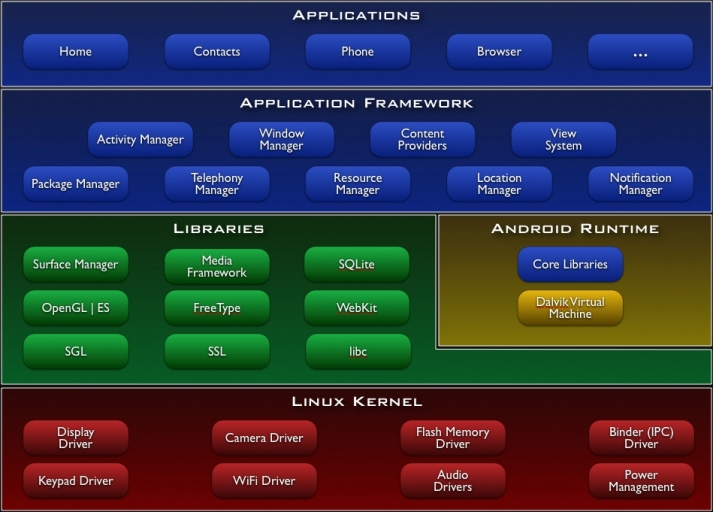
\includegraphics[width=1.0\textwidth]{images/chap4_android_architecture.jpg}
\caption{Android Architecture.}
\label{fig:groupware_taxonomy}
\end{figure}

\subsection{Broadcast}

\subsection{User}

\subsection{Role}

\subsection{Environment}

\section{Collaboration Stack}

\subsection{Ontology of collaboration patterns}

